\documentclass[20pt,margin=1in,innermargin=-4.5in,blockverticalspace=-0.25in]{tikzposter}
\geometry{paperwidth=42in,paperheight=32in}
\usepackage[utf8]{inputenc}
\usepackage{amsmath}
\usepackage{amsfonts}
\usepackage{amsthm}
\usepackage{amssymb}
\usepackage{mathrsfs}
\usepackage{graphicx}
\usepackage{adjustbox}
\usepackage{enumitem}
\usepackage[backend=biber,style=numeric]{biblatex}
\usepackage{uwtheme}
\usepackage{capt-of}
\usepackage{color}
\usepackage{hyperref}


\usepackage{mwe} % for placeholder images

\addbibresource{refs.bib}

% set theme parameters
\tikzposterlatexaffectionproofoff
\usetheme{UWTheme}
\usecolorstyle{UWStyle}

\usepackage[scaled]{helvet}
\renewcommand\familydefault{\sfdefault} 
\usepackage[T1]{fontenc}

%Imported packages
\usepackage{graphicx}
\usepackage{makecell}
\usepackage{tabularx}
\usepackage{multirow}
%\usepackage[table]{xcolor}
%\usepackage[demo]{graphicx}
\usepackage{subfig}
\usepackage{colortbl}

\DeclareMathOperator*{\argmax}{argmax}
\DeclareMathOperator*{\argmin}{argmin}
\usepackage[symbol]{footmisc}
\usepackage{hyperref}
\usepackage{booktabs}

% Color Definitions
\definecolor{earthquake}{HTML}{ffcc99}
\definecolor{flood}{HTML}{94c9ff}
\definecolor{typhoon}{HTML}{99ff99}
\definecolor{attack}{HTML}{f0d16e}
\definecolor{wildfire}{HTML}{ff6666}

% Figures
\newcommand\filledcirc{{\color{blue}\bullet}\mathllap{\bluecirc}}

% Tables
\newcolumntype{L}[1]{>{\raggedright\arraybackslash}p{#1}}
\newcolumntype{C}[1]{>{\centering\arraybackslash}p{#1}}
\newcolumntype{R}[1]{>{\raggedleft\arraybackslash}p{#1}}


\title{DeID-VC: Speaker De-identification via Zero Shot Voice Conversion}

% Title
\author{Ruibin Yuan \quad
        Yuxuan Wu \quad
        Jacob Li \quad
        Jaxter Kim \\
        \texttt{\{ruibiny,yuxuanw2,jacobli,jaxterk\}@andrew.cmu.edu}\\
        %Language Technologies Institute\\
        Carnegie Mellon University}
%%% SAL MOD
\institute{}
\insertlogoi[width=10cm]{cmu-stacked-red.png}
%\insertlogoii[width=15cm]{lti-stacked.png}
\insertlogoii[width=0cm]{cmu-stacked-red.png}

\makeatletter
\newcounter{tablecounter}
\newenvironment{tikztable}[1][]{
  \def \rememberparameter{#1}
  \vspace{10pt}
  \refstepcounter{tablecounter}
  \begin{center}
  }{
    \ifx\rememberparameter\@empty
    \else
    \\[10pt]
    {\small Tab.~\thetablecounter: \rememberparameter}
    \fi
  \end{center}
}
\makeatother

% Begin Document
\begin{document}
\maketitle
\centering
\begin{columns}

	% LEFT COLUMN
	\column{0.32}
	\block{Introduction}{
		%\begin{tikzfigure}[ID-DEID illustration]
		%	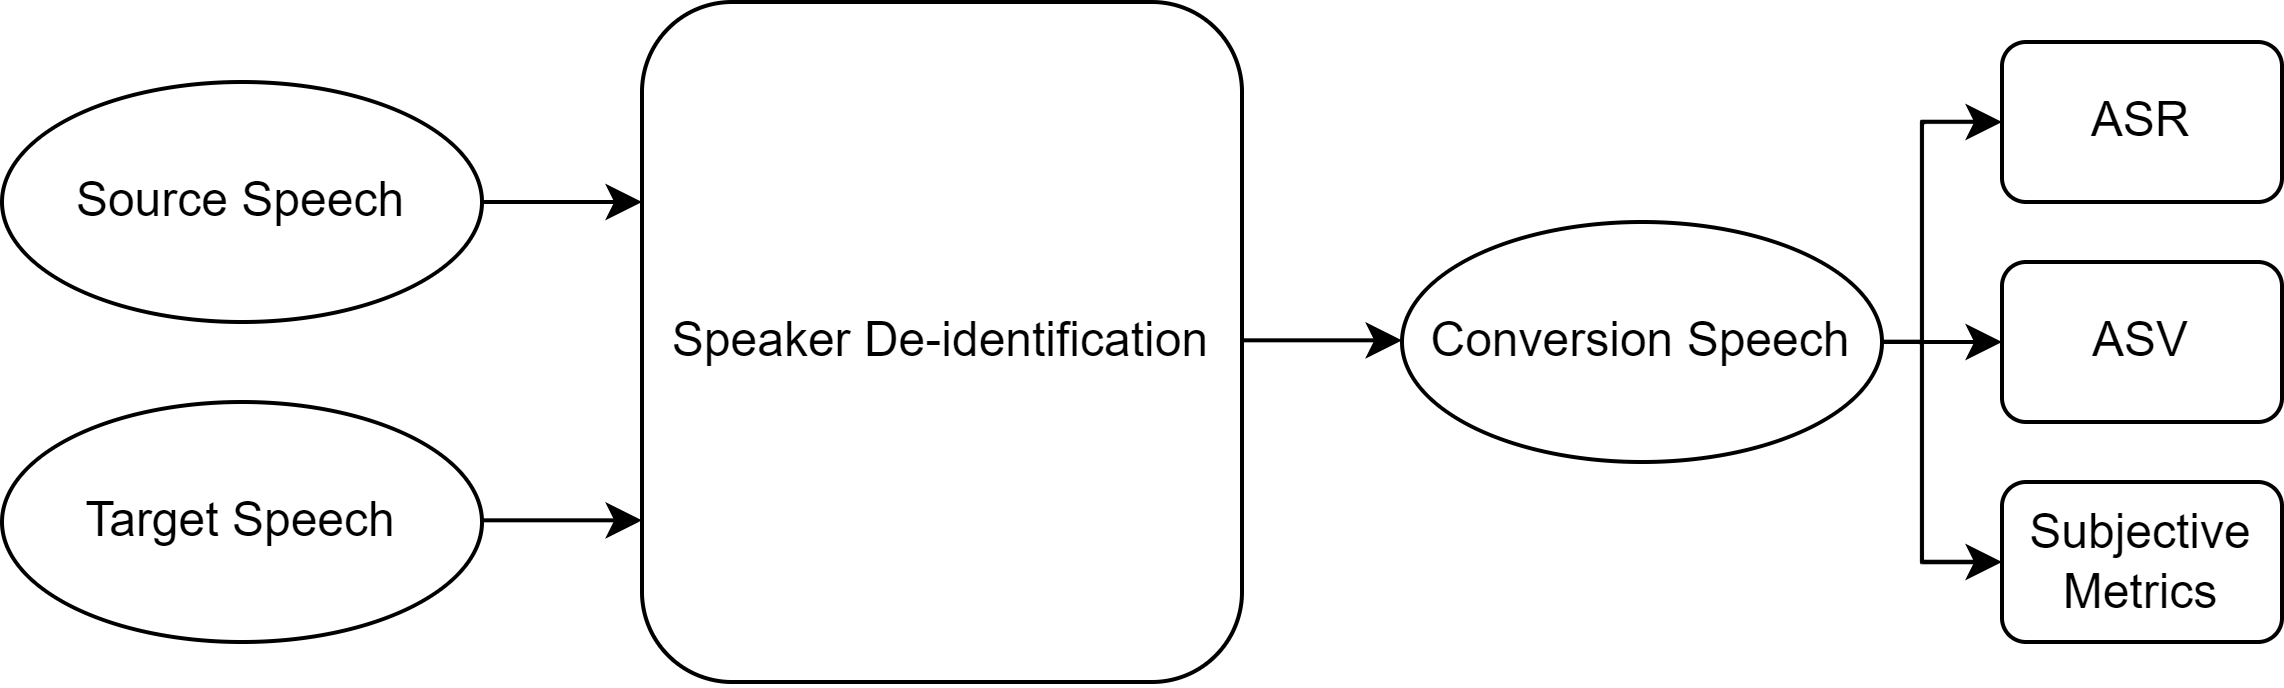
\includegraphics[scale=1.6]{./01-id-deid-illustration.png}
		%\end{tikzfigure}
		\textbf{Speaker De-identification}: Detach the vocal qualities of the speaker, while keeping the original speech contents and intonation, protect user privacy by preventing user being identified from a spoken sound.  

		\textbf{Main Contributions}: 
		    \begin{itemize}
		        \item We propose \textbf{DeID-VC}, a voice conversion Autoencoder for speaker de-identification
		        under zero-shot setting.
		        \item We propose a Pseudo Speaker Generator (\textbf{PSG}) based on Variational Autoencoder (VAE) that enables us to assign unique pseudo speakers to each source speaker.
		        \item We design novel learning objectives to bridge the gap between training and zero-shot inference
		        \item Our method substantially improves intelligibility (WER 10\% lower) and de-identification effectiveness (EER 5\% higher) compared to our baseline.
		    \end{itemize}
	}

	\block{Baseline}{
		\begin{tikzfigure}[Training pipeline (left) and inference pipeline (right) of AutoVC]
			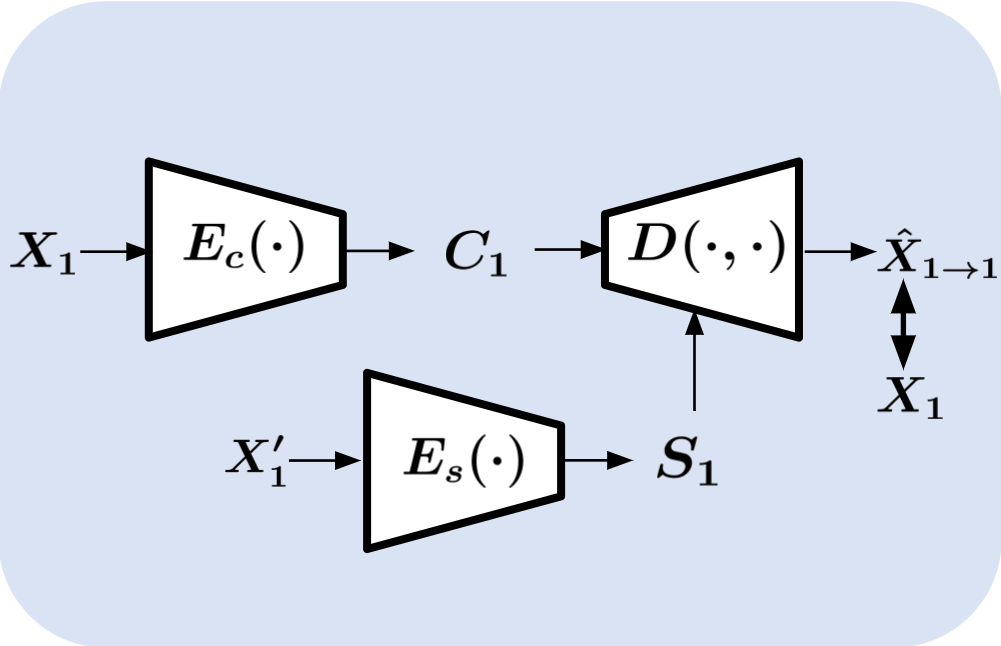
\includegraphics[scale=0.4]{./autovc_train.png}
			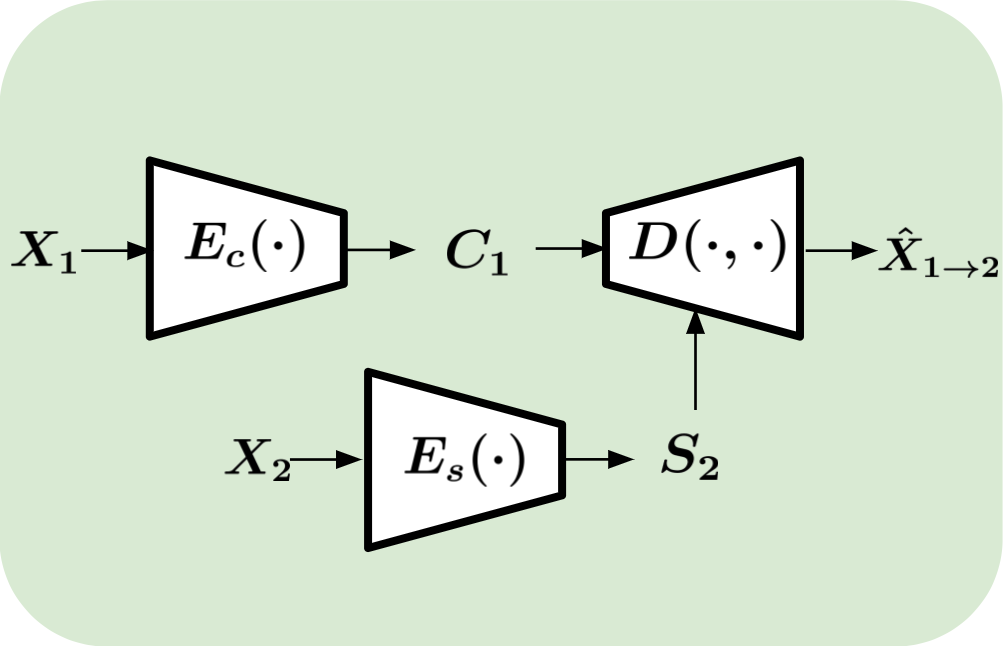
\includegraphics[scale=0.4]{./autovc_infer.png}
		\end{tikzfigure}
	    We use \textbf{AutoVC}[1] as the baseline, an autoencoder with information
		bottleneck to disentangle speaker style and speech content. It contains three parts,
		\begin{itemize}
			\item Content encoder $E_c(\cdot)$ encodes source Mel $X_1$ into content code $C_1$

			\item Speaker encoder $E_s(\cdot)$ encodes target Mel $X_1^{\prime}$ or $X_2$ into target speaker embedding $S$. The target speaker is the same as the source (subscript 1) during training, but different (subscript 2) during inference. 

			\item Decoder $D(\cdot,\cdot)$ combines content code and target speaker embedding to generate converted Mel.
		\end{itemize}
		The training objective $L$ is to minimize the reconstruction losses in terms of raw output, refined output, and content embedding, denoted by $L_{\text{recon}}$, $L_{\text{recon0}}$, $L_{\text{content}}$ respectively.
    \[\min_{E_c(\cdot),D(\cdot,\cdot)} L = L_{\text{recon}} + \mu L_{\text{recon0}} + \lambda L_{\text{content}}\]
    where $\mu$ and $\lambda$ are the weights of corresponding objectives. We use $\mathbb{E}[\cdot]$ to denote the expectation, the three terms are computed by:
    \[L_{\text{recon}} = \mathbb{E}\left[\left\|\hat{X}_{1\rightarrow 1} - X_1\right\|^2_2\right] \]
    \[L_{\text{recon0}} = \mathbb{E}\left[\left\|\tilde{X}_{1\rightarrow 1} - X_1\right\|^2_2\right]\]
    \[L_{\text{content}} = \mathbb{E}\left[\left\|E_c(\hat{X}_{1\rightarrow 1}) - C_1\right\|_1\right]\]
	}

	% CENTER COLUMN
	\column{0.36}
	\block{Our Method}{
		\begin{itemize}
		    \item \textbf{DeID-VC}: We propose DeID-VC, an autoencoder with similar bottleneck
			architecture as AutoVC but with new objectives and a PSG module.
			
			\item \textbf{Objectives for Bridging the Gap}: Model can over-fit leftover speaker identity in $C$, results in performance gap between training and inference. We add a content consistency loss $L_{\text{content\_consist}}$ and a speaker consistency loss $L_{\text{speaker\_consist}}$ to the overall objectives to enable a better disentanglment.
			\begin{align*}
                \min_{E_{c}(\cdot), D(\cdot,\cdot)} L & = L_{\text{recon}} + \mu L_{\text{recon0}} + \lambda L_{\text{content}} + \alpha L_{\text{content\_consist}} + \beta L_{\text{speaker\_consist}}
            \end{align*}
            where $\alpha$ and $\beta$ are the weights of corresponding objectives, and
            \[L_{\text{content\_consist}} = \mathbb{E}\left[\left\lvert E_{c} (\hat{X}_{1\rightarrow 2}) - C_{1}\right\rvert_{1}\right]\]
            \[L_{\text{speaker\_consist}} = \mathbb{E}\left[\left\lvert E_{s} (\hat{X}_{1\rightarrow 2}) - S_{2}\right\rvert_{1}\right]\]
            \begin{tikzfigure}[Training pipeline of DeID-VC. We introduce different target speakers during training by adding new terms.]
     			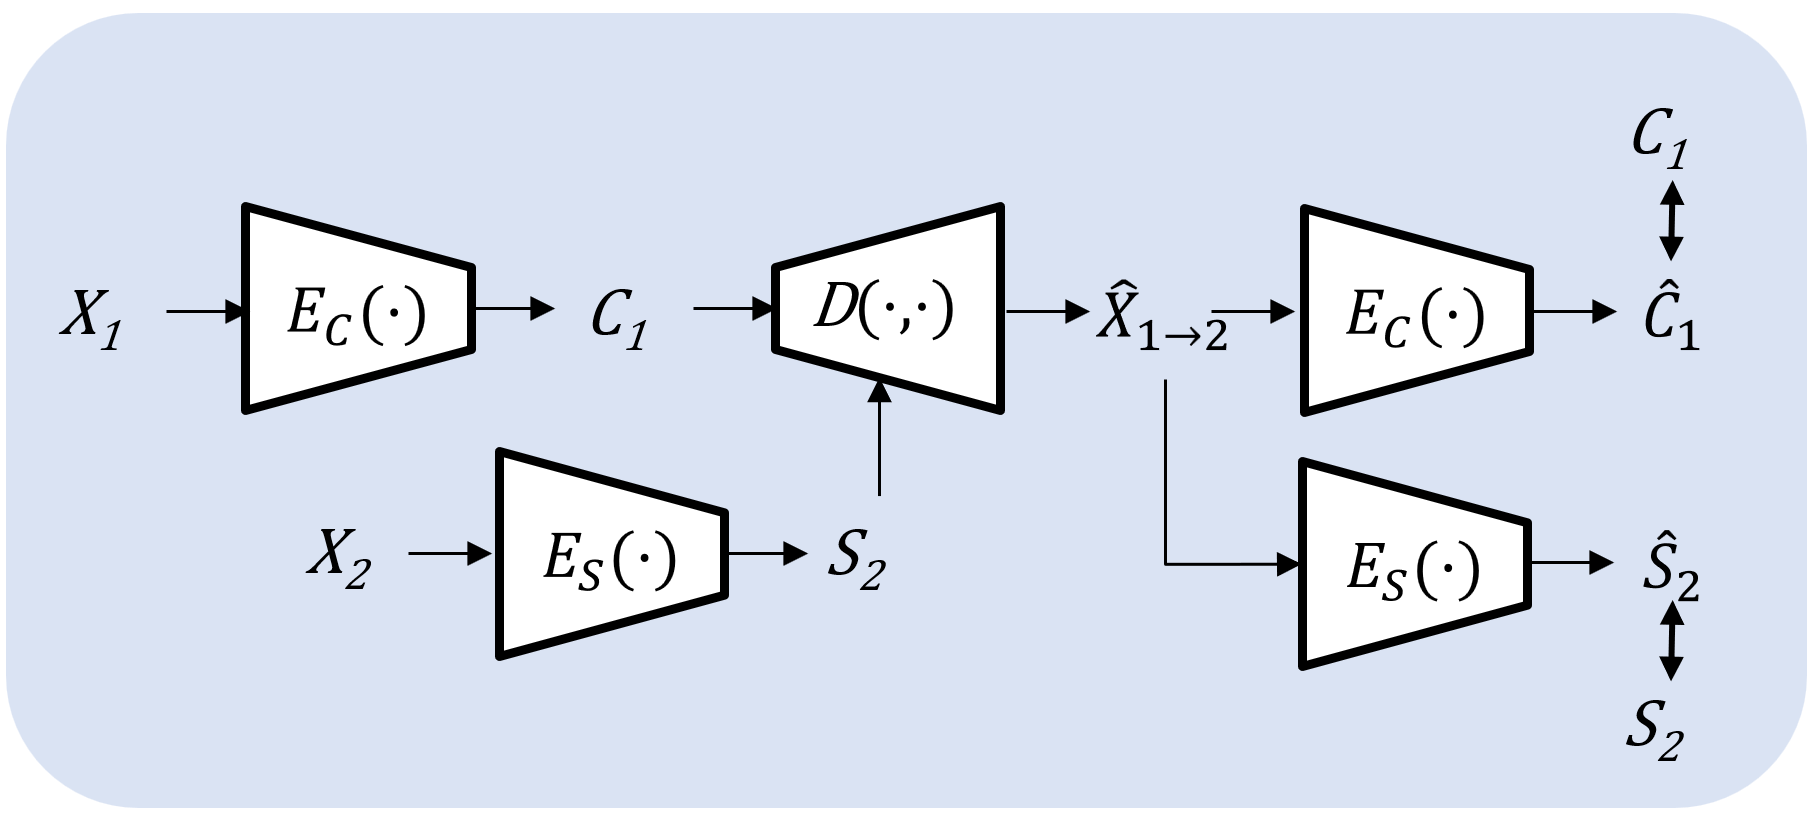
\includegraphics[scale=0.35]{./training_pipeline_DEIDVC.png}
     	    \end{tikzfigure}
     	    
     	    \item \textbf{Pseudo Speaker Generator}: By sampling from noise, the VAE-based PSG allows DeID-VC to produce an arbitrarily large number of realistic pseudo target embeddings in a short time. We replace the $L2$ term of the original VAE loss with a $L1$ term , and add in a cosine distance term $L_{\text{dist}}$. This enhances the convergence of the VAE and allows better modeling of speaker embedding space.
            \begin{tikzfigure}[The PSG is trained in a VAE fashion (left). We can simply replace $E_s(\cdot)$ with PSG during DeID-VC inference (right).]
    			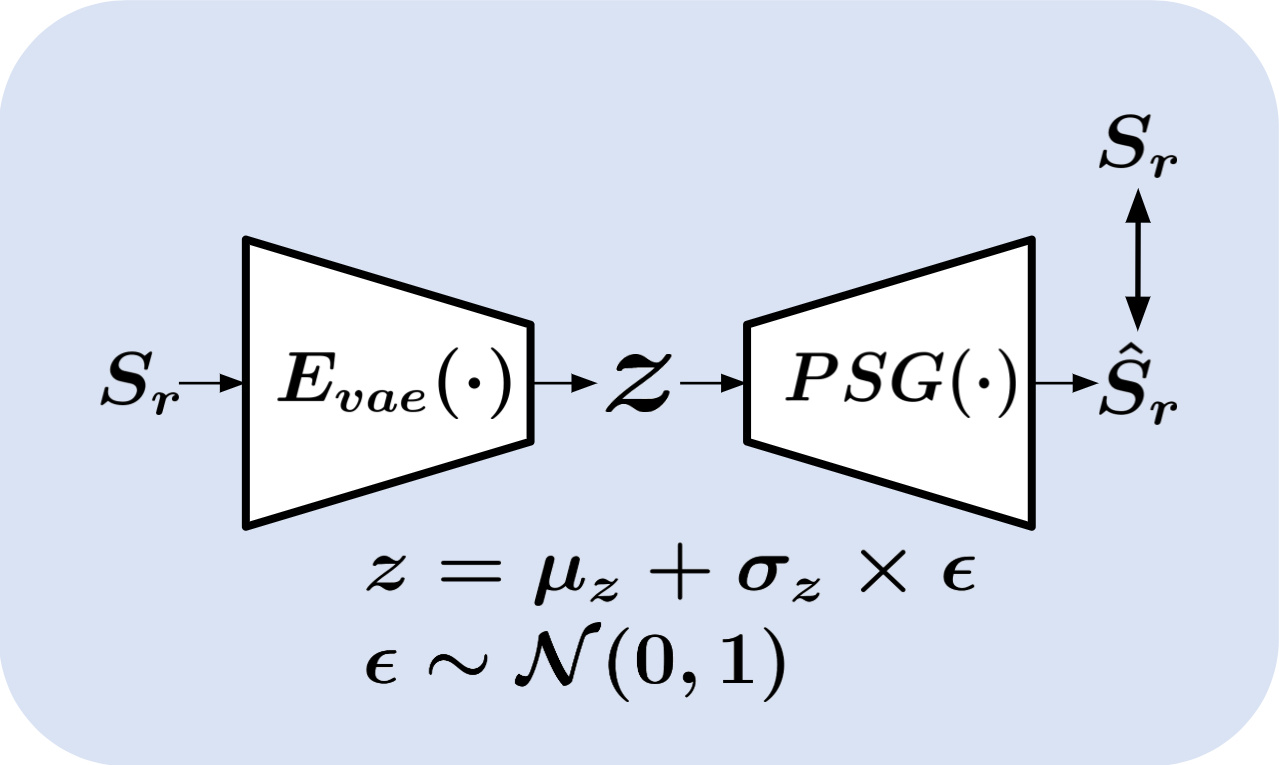
\includegraphics[scale=0.3]{./psg_train.png}
    			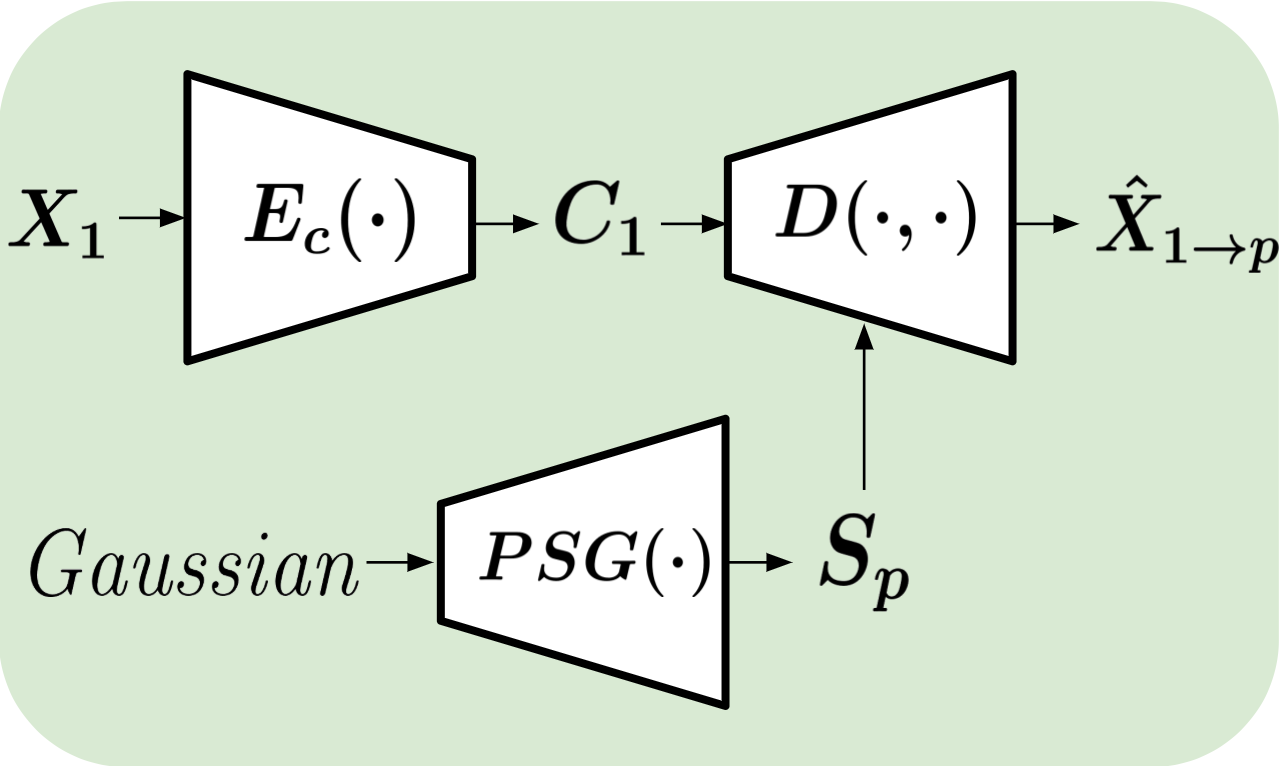
\includegraphics[scale=0.3]{./psg_infer.png}
    		\end{tikzfigure}
			
			\item \textbf{Other Components}: 
			\begin{itemize}
    			\item \textbf{Spectrogram Inverter}: A \textbf{HiFi-GAN}[2] pre-trained on the VCTK corpus as vocoder
    			to reconstruct time domain signals from the Mel-spectrograms.
    
    			\item \textbf{Speaker Encoder}: A LSTM based \textbf{D-Vector} pre-trained on the combination of
    			LibriSpeech and VoxCeleb1 with \textbf{GE2E} loss[3]. 
    
    			\item \textbf{ASR System}: A \textbf{ESPNet}[4] Transformer pre-trained on WSJ corpus, which reaches
    			6.6\% WER on WSJ test\_eavl92.
    
    			\item \textbf{ASV System}: A state of the art \textbf{ECAPA-TDNN}[5] pre-trained on VoxCeleb1+2, which
    			reaches 0.69\% EER on VoxCeleb1-test, and 0.16\% on WSJ corpus.
    		\end{itemize}
    		\end{itemize}
    		
		
	}
    
	% RIGHT COLUMN
	\column{0.32}
	\block{Results}{
        We train and report our baseline and proposed DeID-VC on the combination of WSJ0 and WSJ1. We allocated 60\% of the speakers for training and the remaining 40\% for testing. For the VAE based PSG pre-training part, we use the combination of VoxCeleb 1\&2 for training, VCTK and WSJ for validating.
        \begin{center}
            \begin{tikztable}
                \centering
                \captionof{table}{\textbf{Our Methods Compared to Baseline.} We organize our experiments into four different testing scenarios: \textbf{Seen Source to Unseen Targets (SxU)}, \textbf{Unseen Source to Unseen Targets (UxU)}, \textbf{Seen Source to Pseudo Targets (SxP)}, \textbf{Unseen Source to Pseudo Targets (UxP)}. We evaluate the converted speech with objective metrics: WER, EER, and subjective metrics: MOS in terms of intelligibility, verifiability, and naturalness. We denote $L_{\text{cc}}$ as $L_{\text{content\_consistent}}$, $L_{\text{sc}}$ as $L_{\text{speaker\_consistent}}$. The novel objectives can improve intelligibility and de-identification effectiveness.}
                \label{tab:result}
                \begin{tabular}{c|C{2cm}C{2cm}|C{2cm}C{2cm}C{2cm}C{2cm}|C{2cm}C{2cm}C{2cm}C{2cm}}
                    \hline
                                        & \multicolumn{2}{c|}{Baseline} & \multicolumn{4}{c|}{$+L_{\text{cc}}$} & \multicolumn{4}{c}{$+L_{\text{cc}}+L_{\text{sc}}$} \\
                                        & SxU   & UxU       & SxU   & UxU   & SxP   & UxP       & SxU   & UxU   & SxP   & UxP \\ \hline
                    WER(\%)\downarrow^+ & 42.5  & 48.4      & \textbf{32.8} & \textbf{35.2} & \textbf{30.5} & \textbf{35.7} & 33.3  & 39.9  & 35.9  & 38.4 \\
                    EER(\%)\uparrow^+   & \textbf{41.8} & 36.1      & 40.7  & 36.7  & 41.0  & 37.6      & 41.7  & \textbf{38.4} & \textbf{46.7} & \textbf{38.3} \\ \hline
                    Intelligibility\uparrow^+   & 3.83  & 2.97      & \textbf{4.22} & \textbf{3.72} & \textbf{4.09} & \textbf{3.84}     & 3.94  & 3.50  & 2.81  & 2.78 \\
                    Verifiability\downarrow^+   & 1.88  & 1.63      & \textbf{1.75} & 1.66  & 1.78  & 1.66      & 1.81  & \textbf{1.59} & \textbf{1.50} & \textbf{1.47} \\
                    Naturalness\uparrow^+       & 3.06  & 3.03      & \textbf{4.06} & \textbf{3.44} & \textbf{3.63} & \textbf{3.38}     & 3.56  & 2.78  & 2.72  & 2.34 \\ \hline
                \end{tabular}
            \end{tikztable}
            
            \begin{tikztable}
                \centering
                \captionof{table}{\textbf{Reconstruction Measurement of the VAE.} We compare the reconstructed speaker embeddings with the source embeddings on the training and validation set, in terms of Mean Square Error (MSE) and Cosine Similarity (CosSim), to demonstrate the effectiveness of the specially designed objectives. Our method $L1+L_{\text{dist}}$ achieves better convergence and better modeling of the speaker space.}
                \label{tab:vae eval}
                \begin{tabular}{cC{5cm}C{4cm}C{4cm}C{4cm}}
                \hline
                                                                     &                                      & $L2$     & $L2+L_{\text{dist}}$ & $L1+L_{\text{dist}}$        \\ \hline
                \multicolumn{1}{c|}{\multirow{3}{*}{MSE\downarrow^+}}            & \multicolumn{1}{c|}{Vox(train)} & 0.4044 & 0.4072   & \textbf{0.0831} \\
                \multicolumn{1}{c|}{}                                & \multicolumn{1}{c|}{VCTK(val)}       & 0.6284 & 0.9691   & \textbf{0.5267} \\
                \multicolumn{1}{c|}{}                                & \multicolumn{1}{c|}{WSJ(val)}        & 0.6278 & 0.8421   & \textbf{0.5122} \\ \hline
                \multicolumn{1}{c|}{\multirow{3}{*}{CosSim\uparrow^+}} & \multicolumn{1}{c|}{Vox(train)} & 0.1892 & 0.8698   & \textbf{0.9164} \\
                \multicolumn{1}{c|}{}                                & \multicolumn{1}{c|}{VCTK(val)}       & 0.0905 & 0.4446   & \textbf{0.4972} \\
                \multicolumn{1}{c|}{}                                & \multicolumn{1}{c|}{WSJ(val)}        & 0.0557 & 0.4448   & \textbf{0.5297} \\ \hline
                \end{tabular}
            \end{tikztable}
        \end{center}
    }
    \block{Future Work}{
    - Still needs to improve the intelligibility of zero-shot voice conversion. \\
    - $L2$ loss might not be a reliable measure of speech reconstruction quality, maybe investigate perceptual loss.\\
    - Pre-training with larger data also helps with the intelligibility.
    }
    \block{References and Acknowledgement}{
    \textbf{Thank Prof. Shinji Watanabe, Prof. Ian Lane and Prof. Roger Dannenberg for advising on this paper.}\\
    $[1]$ Qian, Kaizhi, et al. "Autovc: Zero-shot voice style transfer with only autoencoder loss." International Conference on Machine Learning.\\
    $[2]$ Kong, Jungil, Jaehyeon Kim, and Jaekyoung Bae. "Hifi-gan: Generative adversarial networks for efficient and high fidelity speech synthesis."\\
    $[3]$ Wan, Li, et al. "Generalized end-to-end loss for speaker verification."\\
    $[4]$ Watanabe, Shinji, et al. "Espnet: End-to-end speech processing toolkit."\\
    $[5]$ Desplanques, Brecht, Jenthe Thienpondt, and Kris Demuynck. "Ecapa-tdnn: Emphasized channel attention, propagation and aggregation in tdnn based speaker verification."
    }
    

\end{columns}
% End Document
\end{document}
